\section{Une histoire de réflexion}

Dans cette section, l'objectif est de proposer une formulation de la condition en limite en $x=0$ du problème présenté
en figure~\ref{fig:rflx:propa_1D} qui n'impose pas de rajouter une ligne au système d'équations de la FEM.

\begin{figure}[!ht]
	\centering
	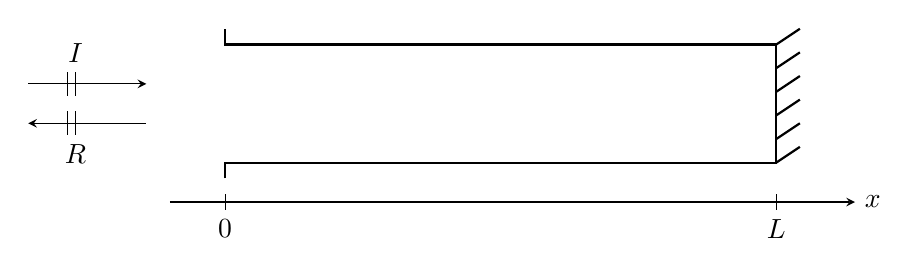
\begin{tikzpicture}[>=stealth]

	% waveguide
	\draw[thick] (0,.3) -- (0,.5) -- (7,.5) -- (7,2) -- (0,2) -- (0,2.2);
	\foreach \i in {0,...,5}{
		\draw[thick] (7,\i*0.3+0.5) -- ++(.3,.2);
	}
	
	% x axis
	\draw[->] (-.7,0) -- (8,0) node[right] {$x$};
	\draw (0,.1) -- ++(0,-.2) node[below] {$0$};
	\draw (7,.1) -- ++(0,-.2) node[below] {$L$};

	% waves
	% R
	\draw[<-] (-2.5,1) -- ++(1.5,0);
	\draw (-2,1.15) -- ++(0,-.3);
	\draw (-1.9,1.15) -- ++(0,-.3) node[below] {$R$};

	% I
	\draw[->] (-2.5,1.5) -- ++(1.5,0);
	\draw (-2,1.65) -- ++(0,-.3);
	\draw (-1.9,1.65) node[above] {$I$} -- ++(0,-.3);

\end{tikzpicture}


	\caption{\label{fig:rflx:propa_1D}Schéma du problème de propagation dans une cavité acoustique 1D de longueur L.}
\end{figure}

\subsection{Partie Théorique}

L'idée est ici de faire apparaitre le vecteur $\ul{u}$ utilisé pour la DGM dans le système
d'équations~\eqref{rflx:governing} régissant le système d'une part et d'exprimer, d'autre part, ce même vecteur avec les
fonction de forme de la FEM et les points de calculs des champs associés.

Dans la suite, le système est considéré unidimensionnel ($\nabla = \frac{\dd}{\dd x}$).

\begin{eqnarray}
	\left\{\begin{array}{l}
		-\nabla p = j\omega\rho v\\
		-\rho c^2\nabla v = j\omega p
	\end{array}\right.
	& \Leftrightarrow &
	\left\{\begin{array}{l}
		j\omega v = -\frac{1}{\rho}\frac{\dd p}{\dd x}\\
		j\omega p = -\rho c^2\frac{\dd v}{\dd x}
	\end{array}\right.\label{rflx:governing}\\
	& \Leftrightarrow &
j\omega \begin{Bmatrix}v\\p\end{Bmatrix} = -\underbrace{\begin{bmatrix}0 & \nicefrac{1}{\rho}\\\rho c^2 & 0
\end{bmatrix}}_{\uul{F}}\frac{\dd}{\dd x}\underbrace{\begin{Bmatrix}v\\p\end{Bmatrix}}_{\ul{u}}\notag\\
	& \Leftrightarrow & \left(j\omega + F\frac{\dd}{\dd x}\right)\ul{u} = \ul{0} \label{rflx:gov_vect}
\end{eqnarray}

Pour découpler les équations, il est alors judicieux de diagonaliser $\uul{F}$, il vient alors (avec $Z_0= \rho c$):

\begin{equation}
	\uul{F} = \uul{W}\uul{\Lambda}\uul{W}^{-1} =
	\begin{bmatrix}
		1 & 1\\
		Z_0 & -Z_0
	\end{bmatrix}
	\begin{bmatrix}
		c & 0\\
		0 & -c
	\end{bmatrix}
	\begin{bmatrix}
		Z_0 & 1\\
		-Z_0 &  1
	\end{bmatrix}\frac{1}{2Z_0} \label{rflx:F_diag}
\end{equation}

En remplaçant~\eqref{rflx:F_diag} dans~\eqref{rflx:gov_vect}, il est alors possible de faire apparaître le vecteur
$\ult{u}$ :

\begin{eqnarray}
	\eqref{rflx:gov_vect} & \Leftrightarrow & j\omega \ul{u} + \uul{W}\uul{\Lambda}\uul{W}^{-1}\ul{u} = 0\notag\\
									    & = & j\omega\uul{W}^{-1} + \uul{\Lambda}\uul{W}^{-1}\ul{u} = 0\notag\\
										& = & j\omega\ult{u} + \uul{\Lambda}\ult{u} = 0\label{rflx:gov_utilde}
\end{eqnarray}

Avec $\ult{u}$ tel que défini en~\eqref{rflx:utilde}.

\begin{equation}
	\ult{u} = \uul{W}^{-1}\ul{u} = \begin{Bmatrix}\tilde{u}^+\\\tilde{u}^-\end{Bmatrix} \label{rflx:utilde}
\end{equation}

Ce vecteur est en fait le vecteur des caractéristiques de l'équation~\eqref{rflx:gov_vect}.

\paragraph{Conditions en $x=0$}

La continuité des pressions acoustiques et vitesses normales à l'entrée du résonateur permet d'écrire le système de
conditions~\eqref{rflx:BC0}.

\begin{equation}
	\left\{\begin{array}{l}
		p(0) = 1 + R\\
		v(0) = \frac{1}{\rho c}(1-R) = \frac{1}{Z_0}(1-R)
	\end{array}\right.\label{rflx:BC0}
\end{equation}

En notant $\ul{u}_0$ le vecteur~$\ul{u}$ précédement introduit pris à la position $x=0$, il vient :

\begin{equation}
	\uul{C}\ul{u}_0 = \uul{C'}\begin{Bmatrix}1\\R\end{Bmatrix} \label{rflx:conditions_set}
\end{equation}

Avec les matrices $\uul{C}$ et $\uul{C'}$ telles que :

\begin{equation*}
	\uul{C} = \uul{I}_2 = \begin{bmatrix}1&0\\0&1\end{bmatrix} \quad,\quad
	\uul{C'} = \begin{bmatrix}\nicefrac{1}{Z_0} & -\nicefrac{1}{Z_0}\\ 1 & 1\end{bmatrix}
\end{equation*}

Pour ré-exprimer l'équation~\eqref{rflx:conditions_set} en fonction des caractéristiques il faut procéder comme suit :

\begin{equation*}
\underbrace{\uul{C}\uul{W}}_{\uult{C}}\uul{W}^{-1}\ul{u}_0 = \uul{C'}\begin{Bmatrix}1\\R\end{Bmatrix}
\end{equation*}

De là, il est possible d'exprimer facilement le vecteur $\ult{u}$ en fonction des deux matrices du jeu de conditions
limites :

\begin{equation*}
\uult{C}\ult{u} = \uul{C'}\begin{Bmatrix}1\\R\end{Bmatrix} \Leftrightarrow \ult{u}_0 = \uult{C}^{-1}\uul{C'}\begin{Bmatrix}1\\R\end{Bmatrix}
\end{equation*}

Sachant que $\uul{C} = \uul{I}_2$ alors $\uult{C} = \uul{W} \Leftrightarrow \uult{C}^{-1} = \uul{W}^{-1}$ et cette
dernière matrice à déjà été exprimée à l'équation~\eqref{rflx:F_diag}.

De là, il vient :

\begin{eqnarray}
	\ult{u}_0 & = & \frac{1}{2Z_0}
					\begin{bmatrix}Z_0 & 1\\-Z_0 & 1\end{bmatrix}
					\begin{bmatrix}\nicefrac{1}{Z_0} & - \nicefrac{1}{Z_0}\\1 & 1\end{bmatrix}
					\begin{Bmatrix}1\\R\end{Bmatrix}\notag\\
	\Leftrightarrow \ult{u} & = & \frac{1}{2Z_0}
					\begin{bmatrix}2&0\\0&2\end{bmatrix}
					\begin{Bmatrix}1\\R\end{Bmatrix}\notag\\
	\Leftrightarrow &&
			\left\{\begin{array}{l}
				\tilde{u}_0^+ = \nicefrac{1}{Z_0}\\
				\tilde{u}_0^- = \nicefrac{R}{Z_0}
		 	\end{array}\right.
\end{eqnarray}

\paragraph{Approximation des caractéristiques}

Le dernier bloc manquant désormais est l'expression des caractéristique en fonction des fonctions de forme associées à
la formultation FEM.

En réutilisant le vecteur des pressions à chaque extrémité du premier élément (tel qu'introduit à la
section~\ref{FEM1D:subsection:linear}) il est possible d'écrire la pression en $x=0$ en faisant usage des fonctions de
forme, ainsi :

\begin{equation*}
	p(0) = \phi_1\GP_0 + \phi_2\GP_1
\end{equation*}

En utilisant l'équation d'Euler, il est ensuite possible de passer à la valeur de la vitesse en $x=0$ :

\begin{equation*}
	j\omega\rho v(0) = -\frac{\dd p}{\frac x} \Rightarrow v(0) = \frac{-1}{j\omega\rho}\left(\phi_1'\GP_0 +
		\phi_2'\GP_1\right)
\end{equation*}

De là, on peut ré-écrire le vecteur $\ul{u}_0$ utilisé pour l'écriture des conditions en fonction des fonctions de forme
:

\begin{equation}
\begin{Bmatrix}v(0)\\p(0)\end{Bmatrix} = \ul{u}_0 = \begin{bmatrix} -\nicefrac{\phi_1'}{j\omega\rho} &
-\nicefrac{\phi_2'}{j\omega\rho}\\\phi_1&\phi_2\end{bmatrix}\begin{Bmatrix}\GP_0\\\GP_1\end{Bmatrix}
	\label{rflx:u_shapefun}
\end{equation}


TO BE CONTINUED


\begin{figure}[!ht]
	\centering
	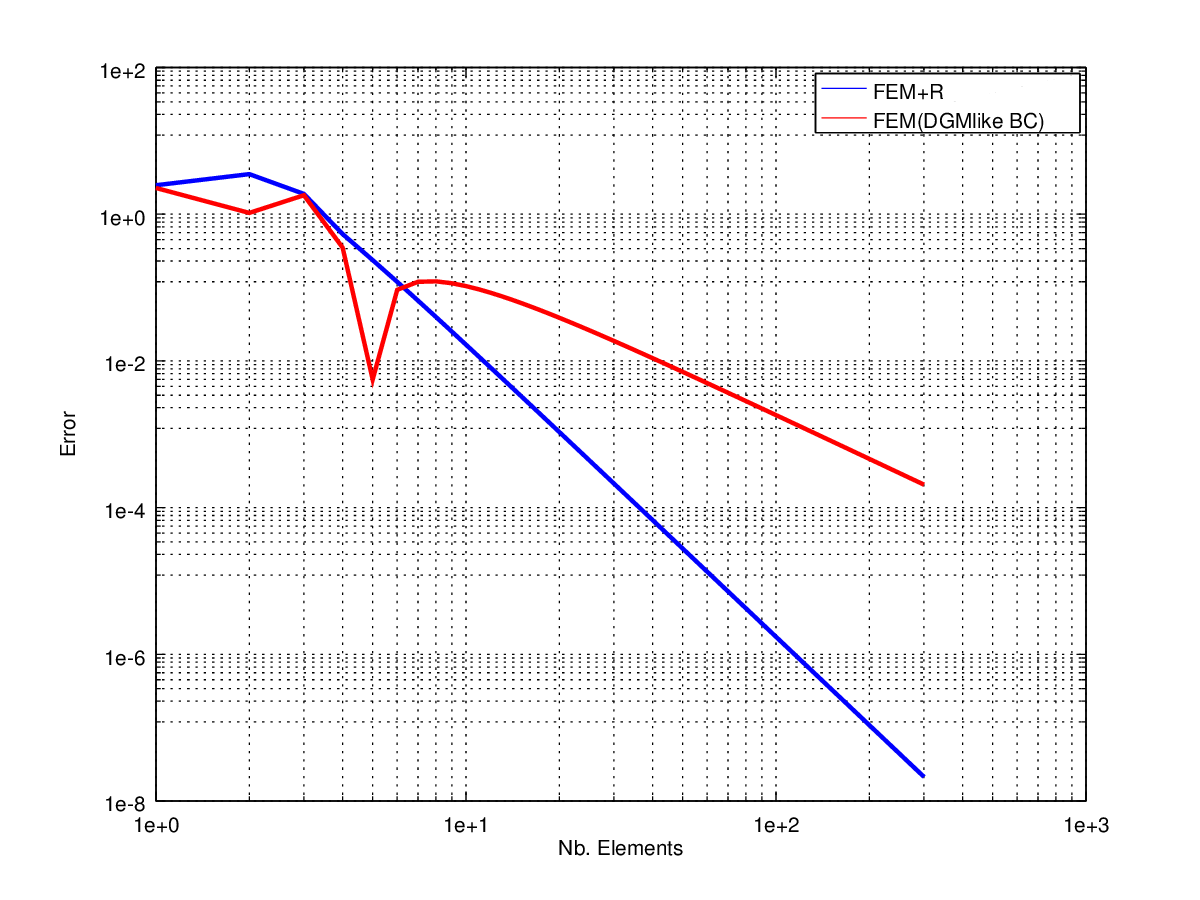
\includegraphics[width=\textwidth]{figs/FEM/DGMlike/convergence.png}
	\caption{Comparaison de l'erreur commise en fonction du nombre de points pour une méthode FEM+R en bleu et
	FEM+formulation DGM en rouge.}
\end{figure}
